\documentclass[11pt, a4paper]{article}
\usepackage[utf8]{inputenc}
\usepackage[spanish]{babel}
\usepackage{amsmath}
\usepackage{amsfonts}
\usepackage{amssymb}
\usepackage{graphicx}
\usepackage{geometry}
\usepackage{booktabs}
\usepackage{hyperref}
\usepackage{tabularx}
\usepackage{enumitem}
\usepackage{setspace}

% Code listings 
\usepackage{listings}
\usepackage{xcolor}

% Code listings style 
\definecolor{codegreen}{rgb}{0,0.6,0}
\definecolor{codegray}{rgb}{0.5,0.5,0.5}
\definecolor{codepurple}{rgb}{0.58,0,0.82}
\definecolor{backcolour}{rgb}{0.95,0.95,0.92}
\lstdefinestyle{mystyle}{
    backgroundcolor=\color{backcolour},   
    commentstyle=\color{codegreen},
    keywordstyle=\color{magenta},
    numberstyle=\tiny\color{codegray},
    stringstyle=\color{codepurple},
    basicstyle=\ttfamily\footnotesize,
    breakatwhitespace=false,         
    breaklines=true,                 
    captionpos=b,                    
    keepspaces=true,                 
    % numbers=left,                    
    % numbersep=5pt,                  
    showspaces=false,                
    showstringspaces=false,
    showtabs=false,                  
    tabsize=2
}
\lstset{style=mystyle}
\renewcommand{\lstlistingname}{Algoritmo}

% Diagrams
\usepackage{tikz}
\usepackage{etoolbox}
\usepackage{pgfplots}
\usepackage{ifthen}
\pgfplotsset{compat=1.12}

\usetikzlibrary{decorations}
\usetikzlibrary{decorations.pathreplacing}
\usetikzlibrary{calc}
\usetikzlibrary{positioning}
\usetikzlibrary{arrows}
\usetikzlibrary{matrix}
\usetikzlibrary{fit}

\usepackage[table]{xcolor}
\usepackage{caption}
\usepackage{array}

\usepackage[numbers]{natbib}

\hypersetup{
    colorlinks=true,
    linkcolor=blue,
    filecolor=magenta,      
    urlcolor=blue,
    citecolor=blue,
    pdftitle={Overleaf Example},
    pdfpagemode=FullScreen,
}

\title{
    {Trabajo Inteligencia Empresarial} \\
    {\large Transporte Vehicular en Montevideo}
}

\author{Guillermo Golpe, Federico Vareika}
\date{2026}

\begin{document}

\maketitle

\newpage

\tableofcontents

\newpage

\section{Introducci\'on}

Este trabajo presenta un proyecto de Inteligencia de Negocios (BI) enfocado en 
analizar el transporte vehicular en la ciudad de Montevideo durante el año 2022
. El objetivo principal es procesar y unificar distintos conjuntos de datos, 
específicamente mediciones de velocidad promedio, conteo vehicular y 
siniestros de tránsito, para generar información útil. A través de este 
análisis, se busca entender cómo fluye el tráfico en la ciudad, evaluar la 
eficiencia de las avenidas y medir el peligro real de las distintas zonas 
relacionando los accidentes con el volumen de autos.

Para lograrlo, se armó un proceso de Extracción, Transformación y Carga (ETL) 
en Python que limpia los datos crudos y los organiza en un modelo de esquema 
estrella. Sobre esta base, se calculan métricas clave como el Índice de 
Eficiencia y el Índice de Riesgo, y se utilizan algoritmos como K-Means para 
clasificar los puntos críticos. Finalmente, todos los resultados y las 
recomendaciones, como la asignación de prioridades para instalar nuevos radares,
se muestran en reportes interactivos en Power BI para facilitar la lectura y 
la toma de decisiones. 






\section{Arquitectura de Datos: Proceso de Extracción, Transformación y Carga (ETL)}

Para procesar los datos, usamos un modelo de Esquema de Constelaci\'on,
y luego para el an\'alisis, juntamos todos los datos para la tabla del
an\'alisis correspondiente. 
La idea es tener una buena base para poder analizar con python 
de manera eficiente. Las tablas estandarizadas est\'an separadas en
tablas de dimensi\'on (\texttt{dim\_*.csv}) y tablas de hechos 
(\texttt{fact\_*.csv}).

\subsection{Carga de datos}

Los datasets usados son los siguientes:
\begin{itemize}[noitemsep]
    \item \href{https://catalogodatos.gub.uy/dataset/velocidad-promedio-vehicular-en-las-principales-avenidas-de-montevideo}{Velocidad promedio}
    \item \href{https://catalogodatos.gub.uy/dataset/conteo-vehicular-en-las-principales-avenidas-de-montevideo}{Conteo vehicular}
    \item \href{https://catalogodatos.gub.uy/dataset/base-anual-de-personas-lesionadas-en-siniestros-de-transito}{Lesionados en siniestros}
\end{itemize}

La carga de datos se realiza autom\'aticamente con el script \texttt{descargar\_con\_fechas.py}.

\subsection{Construcción de Dimensiones (\texttt{build\_dim\_*.py})}

Los módulos de dimensión procesan los datos crudos para extraer entidades
descriptivas, normalizar sus atributos y asignarles claves 
(IDs numéricos enteros). 
Este proceso garantiza la integridad referencial del modelo de datos y elimina
la redundancia de datos almacenados.

\subsubsection*{Script: \texttt{build\_dim\_calle.py}}
Este script genera un catálogo único y estandarizado de todas las calles de la
ciudad. 
Toma como entrada la dimensión de ubicaciones base y extrae la columna
descriptiva original, la cual frecuentemente contiene cadenas compuestas de 
intersecciones viales (ej. ``Avenida A / Calle B'' o ``Calle C esq. Calle D'').

El procesamiento ejecuta las siguientes limpiezas:
\begin{itemize}[noitemsep]
    \item \textbf{Fragmentación de Cadenas}: 
        Divide el texto iterando sobre delimitadores como `` / '' y `` esq. ''.
    \item \textbf{Estandarización de Texto}:
        Elimina espacios en blanco residuales y lleva todo el texto a letras 
        mayúsculas.
    \item \textbf{Filtrado de Anomalías}:
        Aplica una expresión regular 
        (\textrm{r`\string^-?\textbackslash d+\textbackslash.?\textbackslash d*\$'}) 
        para detectar y descartar fragmentos que consisten puramente en números,
        los cuales representan errores de tipeo o marcadores kilométricos 
        inválidos como nombres de calles.
    \item \textbf{Indexación}: 
        Agrupa los valores para asegurar la unicidad y asigna un identificador
        secuencial (\texttt{calle\_id}), exportando el resultado al archivo
        \texttt{dim\_calle.csv}.
\end{itemize}

\subsubsection*{Script: \texttt{build\_dim\_fecha.py}}

Este script crea una tabla de calendario completa para desglosar cualquier fecha
por año, mes o día. 
No asume un solo formato de datos porque los archivos del gobierno siempre
varían en ese sentido.
\begin{itemize}[noitemsep]
    \item \textbf{Consolidación Multi-Fuente}:
        Itera sobre los directorios de velocidad, conteo vehicular y siniestros.
        Para los siniestros, aplica un mapeo de columnas específico 
        (SIN\_MAPPING) debido a discrepancias en el esquema de origen.
    \item \textbf{Conversión Temporal}:
        Convierte el texto crudo al tipo datetime.
    \item \textbf{Derivación de Atributos}:
        Tras obtener un listado único y cronológico de todas las fechas 
        registradas, el algoritmo extrae directamente del objeto datetime tres 
        nuevas columnas de análisis: el año (anio), el mes numérico (mes) y el 
        día (dia). Finalmente, asigna una clave primaria.
\end{itemize}

\subsubsection*{Script: \texttt{build\_dim\_detector.py}}
\begin{itemize}[noitemsep]
    \item \textbf{Extracción de Metadata}:
        Selecciona el código natural del detector y sus descriptores geográficos
        (avenida, intersección anterior e intersección siguiente).
    \item \textbf{Casteo de Precisión}:
        Fuerza la conversión de los tipos de datos de latitud y longitud a
        Float64 explícitamente.
    \item \textbf{Renombramiento Estructural}:
        Limpia los nombres de las columnas, eliminando prefijos innecesarios 
        (\texttt{dsc\_}), y exporta la tabla única de sensores con su 
        respectivo ID.
\end{itemize}

\subsubsection*{Script: \texttt{build\_dim\_ubicacion.py}}

Este script unifica dos tipos de coordenadas a uno, consolidando los datos en
una tabla diferenciada por el \texttt{tipo}.
\begin{itemize}[noitemsep]
    \item \textbf{Procesamiento de Coordenadas GPS}: 
        Para los datos de flujo vehicular, extrae directamente la latitud y
        longitud y asigna el identificador categórico \texttt{tipo = `avenida'}.
    \item \textbf{Transformación de Coordenadas UTM}:
        El dataset de siniestros no provee latitud y longitud, sino coordenadas
        planas en formato UTM (x, y). 
        El script usa la funci\'on \texttt{utm\_to\_latlon} para pasar de UTM a 
        latitud y longitud. 
        A estos puntos les asigna el indicador \texttt{tipo = `calle\_siniestro'}.
    \item \textbf{Agrupación y Fusión de Descripciones}:
        Consolida todos los puntos en un único DataFrame.
        Si múltiples sensores o accidentes comparten las mismas coordenadas, 
        agrupa el registro fusionando las descripciones de texto para no 
        perder contexto, asignando luego la llave primaria final.
\end{itemize}

\subsection{Construcción de Hechos (\texttt{build\_fact\_*.py})}

Los módulos de hechos se encargan de consolidar el volumen alto de datos del
sistema. Su función principal es reemplazar los datos que ya consolidamos en 
las tablas de dimensi\'on por los identificadores correspondientes.

\subsubsection*{Script: \texttt{build\_fact\_medicion.py}}
\begin{itemize}[noitemsep]
    \item \textbf{Cruce de Orígenes}:
        En cada iteración mensual, normaliza los textos de fecha y extrae la
        hora y el minuto como números enteros. Utiliza una llave compuesta de 5
        variables (\texttt{[`fecha', `hora', `minuto', `cod\_detector', `id\_carril']}) 
        para ejecutar un Left Join, la velocidad promedio de un vehículo con
        el volumen de la calle en ese minuto exacto.
    \item \textbf{Reconstrucción Temporal}:
        Concatena las variables de hora y minuto que estaban separadas en un
        formato de texto estructurado (\texttt{"HH:MM:00"}) y lo convierte en
        un tipo de dato nativo de tiempo (\texttt{hora\_t}).
    \item \textbf{Mapeo de Claves y Streaming}:
        Cruza el resultado con las dimensiones en memoria para obtener
        el \texttt{fecha\_id} y \texttt{detector\_id}. Elimina todas las 
        columnas descriptivas dejando solo números. 
\end{itemize}

\subsubsection*{Script: \texttt{build\_fact\_siniestros.py}}

Se encarga de modelar la tabla de transacciones de accidentes de tránsito, 
conectando la metadata categórica del siniestro con las dimensiones espacial
y temporal.
\begin{itemize}[noitemsep]
    \item \textbf{Estandarización de Esquema y Texto}: 
        Primero, se cargan los datos y se utiliza el diccionario SIN\_MAPPING
        para renombrar las columnas y ajustarlas a la convención definida en el
        proyecto. 
        Adicionalmente, se aplica una limpieza (\textit{strip}) a 
        las columnas de texto para eliminar cualquier espacio en blanco
        innecesario al inicio o al final de las palabras.
    \item \textbf{Geoprocesamiento Integrado}:
        Al igual que la dimensión de ubicación, este script de hechos repite la
        transformación geométrica \texttt{utm\_to\_latlon}.
    \item \textbf{Cruces}:
        Ejecuta un cruce conectando la fecha del siniestro con
        \texttt{dim\_fecha}, y un cruce espacial sobre la latitud y longitud 
        para recuperar el \texttt{ubicacion\_id} generado en la etapa de 
        dimensiones.
    \item \textbf{Limpieza Final y Exportación}:
        Desecha las coordenadas crudas y las fechas en formato texto, 
        preservando únicamente las claves (\textit{IDs}) y las
        variables del accidente (si el conductor 
        utilizaba casco o cinturón, sexo, edad, tipo de siniestro). 
\end{itemize}


\section{Analítica Espacial}

\subsection{Métricas y Utilidad}

Este script calcula dos métricas principales para el manejo del tráfico: el 
Índice de Eficiencia y el Índice de Riesgo. El Índice de Eficiencia es una 
métrica que mide qué tan bien fluye el tráfico en un tramo específico, 
relacionando su capacidad de absorber un alto volumen de vehículos mientras 
mantiene una velocidad promedio óptima. Esto es muy útil para la toma de 
decisiones, ya que permite identificar qué avenidas están funcionando 
bajo su potencial y cuáles manejan un buen flujo de tráfico.

Por otro lado, el Índice de Riesgo analiza la seguridad de forma 
proporcional al volumen de tr\'afico. 
En vez de solo contar cuántos accidentes hay en una calle, este índice compara 
la cantidad de siniestros con el volumen total de tráfico que circula por el 
mismo lugar. 
Este enfoque es fundamental para analizar el peligro real de una ubicaci\'on.

\subsection{Lógica General}

\subsubsection*{Cargar Datos}

Importar las tablas de dimensi\'on 
\texttt{dim\_detector.csv} y
\texttt{dim\_ubicacion.csv}, y hechos
\texttt{fact\_medicion.csv} y
\texttt{fact\_siniestros.csv}.

\subsubsection*{Agregar Métricas de Tráfico}
\begin{itemize}[noitemsep]
    \item Agrupar la información de la tabla de mediciones utilizando el 
        identificador de cada detector.
    \item Calcular la velocidad media histórica y sumar el volumen total de 
        vehículos para cada detector.
\end{itemize}

\subsubsection*{Asignación Espacial de Siniestros}
\begin{itemize}[noitemsep]
    \item Iterar sobre cada uno de los siniestros registrados.
    \item Utilizar la fórmula de distancia Haversine para obtener la 
        distancia geográfica entre la ubicación del accidente y todos 
        los detectores de la ciudad.
    \item Identificar cuál es el detector más cercano al lugar del siniestro.
    \item Si la distancia al detector más cercano es inferior a 500 metros, 
        asignar ese siniestro a dicho detector.
    \item Agrupar los siniestros asignados y contabilizar el total por cada 
        detector, uniendo este resultado a los datos de tráfico previos.
\end{itemize}

\subsubsection*{Cálculo de Índices Normalizados}
\begin{itemize}[noitemsep]
    \item Normalizar los valores de volumen y velocidad, dividiendo cada 
        registro por el valor máximo histórico encontrado para llevarlos a una 
        escala estandarizada de 0 a 1.
    \item Calcular el Índice de Eficiencia multiplicando el volumen 
        normalizado por la velocidad normalizada, y ajustando a una escala 
        base 100.
    \item Calcular el Riesgo Inicial dividiendo la cantidad de siniestros 
        entre el volumen normalizado.
    \item Calcular el Índice de Riesgo final normalizando el riesgo inicial 
        contra el máximo riesgo detectado, ajustando nuevamente a una escala 
        base 100.
\end{itemize}

\subsubsection*{Exportar Resultados}
\begin{itemize}[noitemsep]
    \item Guardar la tabla final en el archivo 
        \texttt{tramos\_analitica\_2022.csv}. 
        El resultado generado es un archivo base que contiene un registro 
        único por cada detector (avenida/calle).
    \item Las columnas que se generan consolidan tanto la estadística cruda 
        (\texttt{cantidad\_siniestros}, \texttt{volumen\_total}, 
        \texttt{velocidad\_media}) como los dos nuevos indicadores creados 
        (\texttt{indice\_eficiencia}, \texttt{indice\_riesgo}).
\end{itemize}

Este archivo concluye la fase de procesamiento espacial y sirve como tabla 
maestra (o dimensión enriquecida) para alimentar los gráficos principales y 
mapas geográficos básicos en Power BI.

\subsection{Reporte}

\begin{figure}[ht]
    \centerline{
        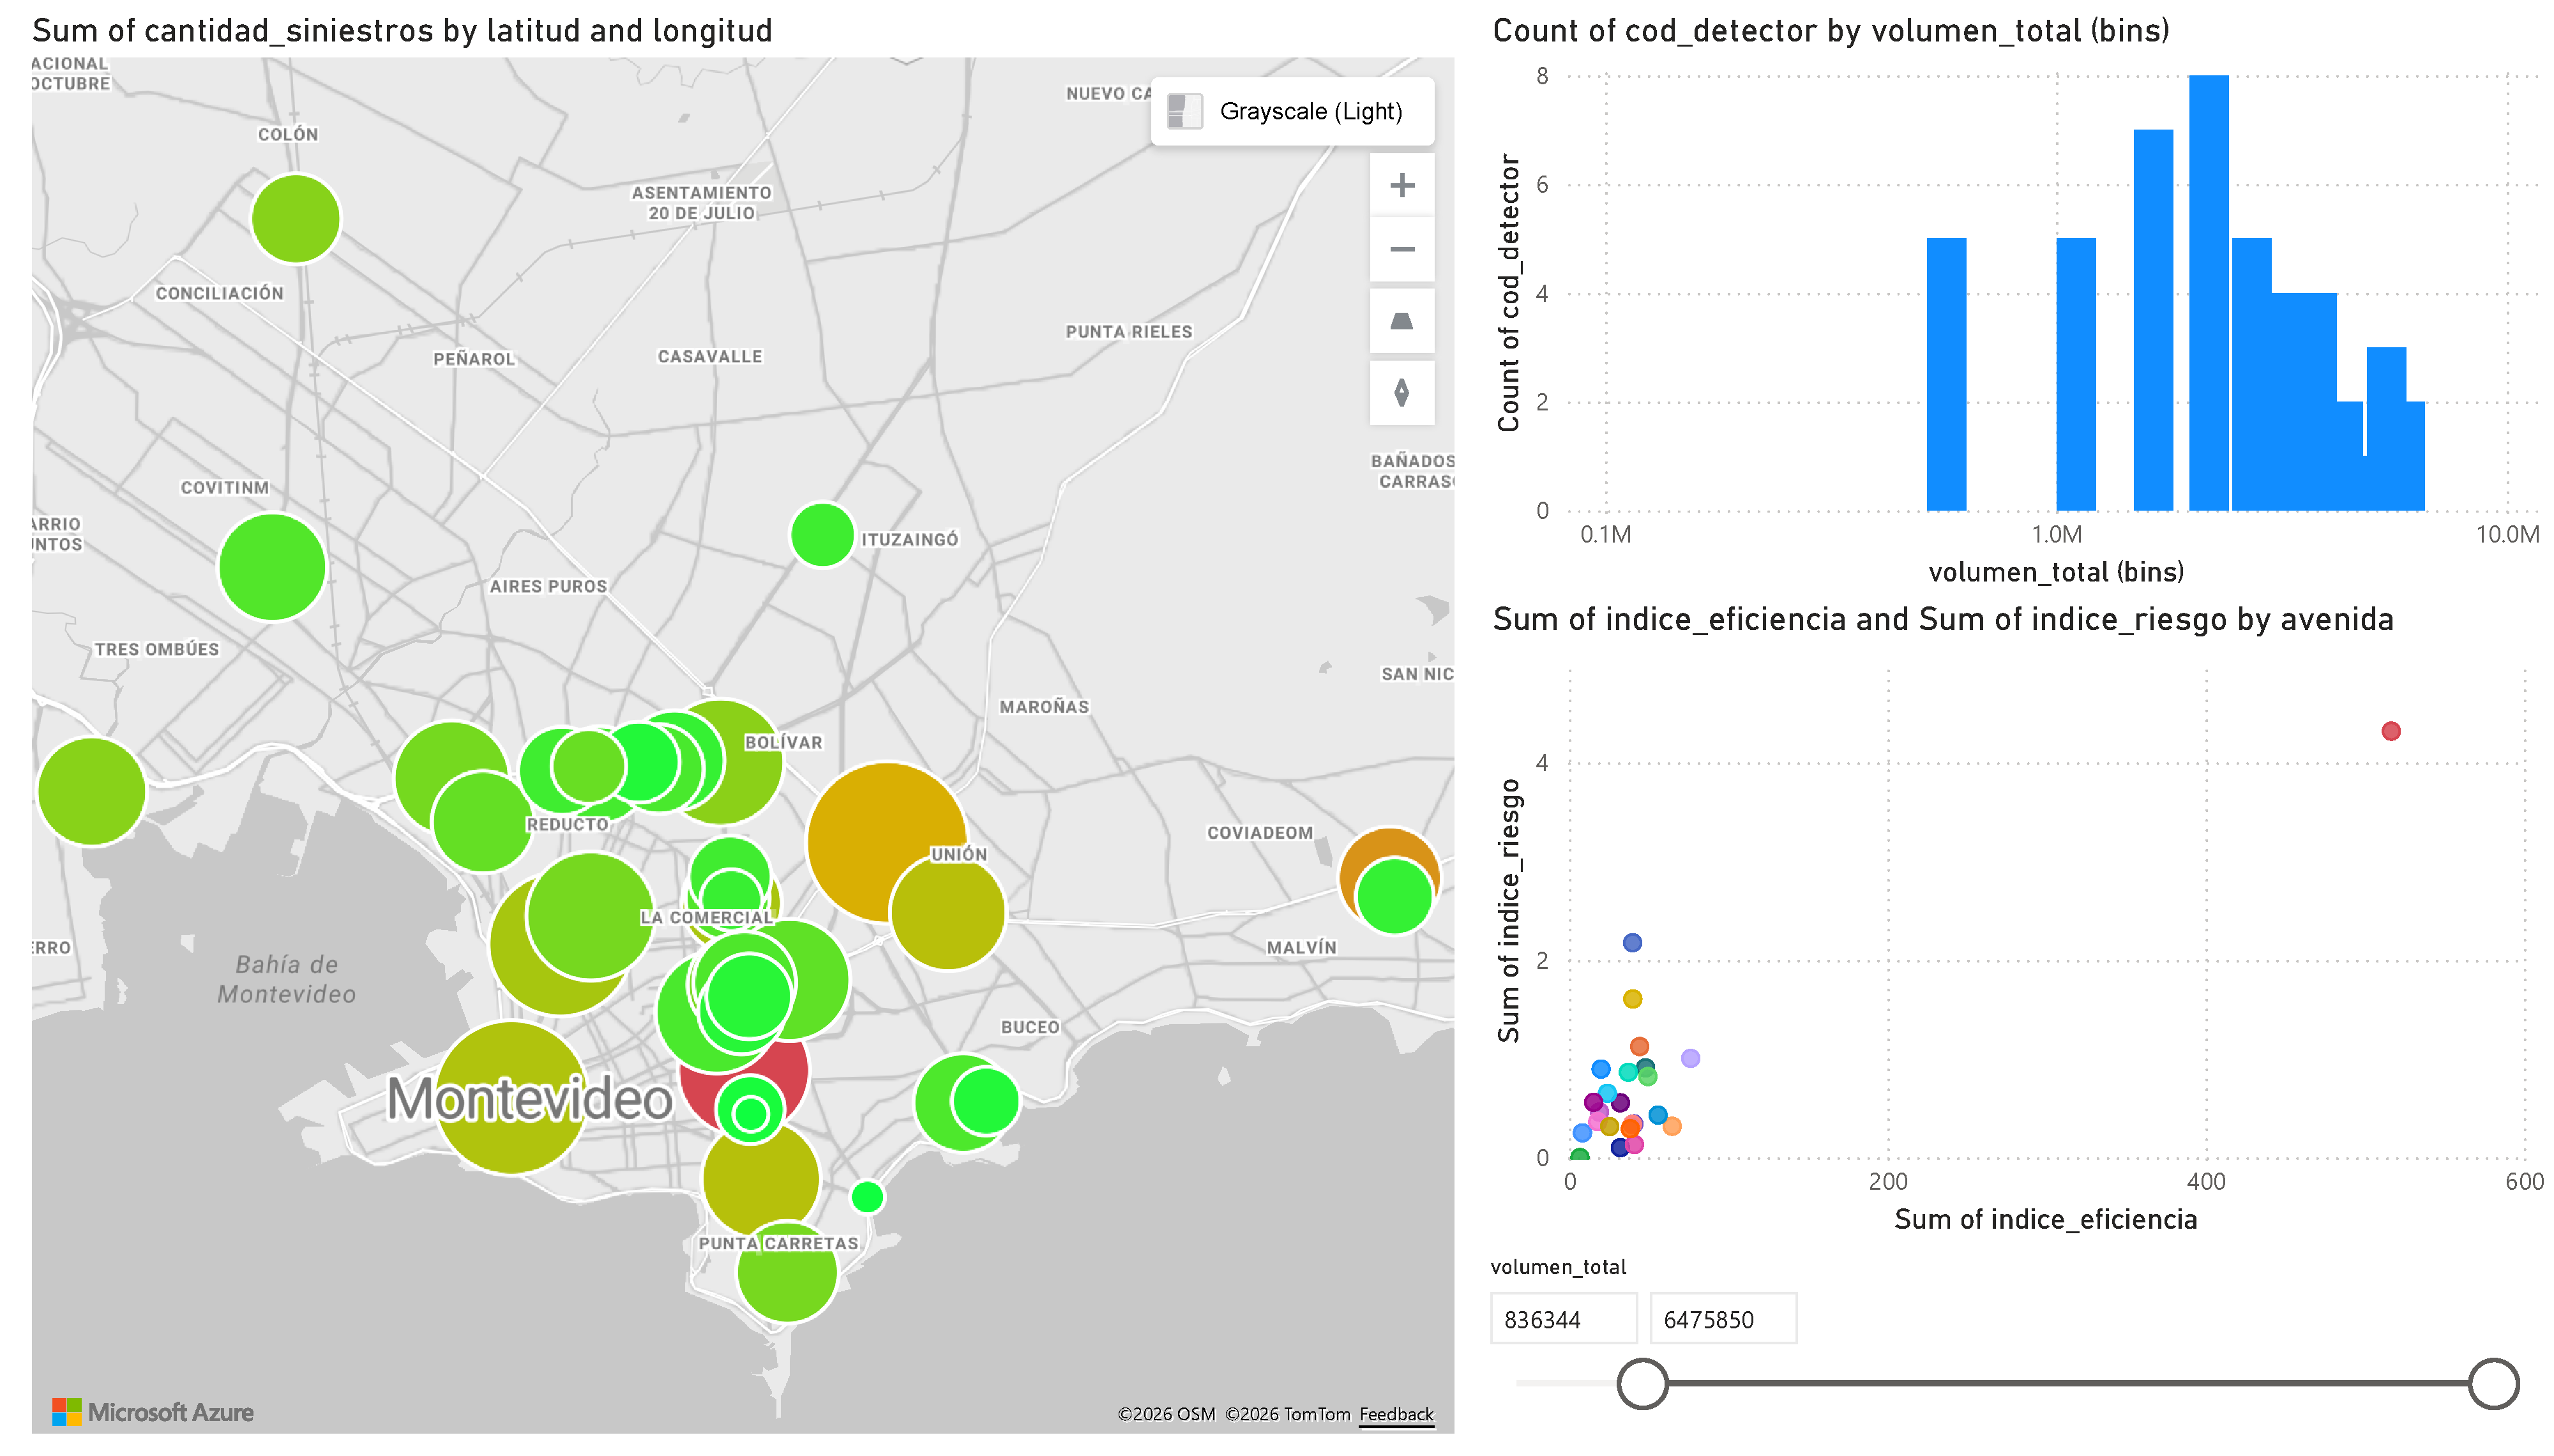
\includegraphics[page=1, scale=0.25]{graphics/reporte.pdf}
    }

    \caption{
        Reporte de las anal\'iticas iniciales: \\
        (\textbf{izquierda}) Mapa de cantidad de siniestros en cada zona 
            (detector). 
        (\textbf{arriba-derecha}) Histograma mostrando la distribuci\'on de 
            detectores seg\'un el volumen de autos medido. Notar que es una 
            escala logar\'itmica.
        (\textbf{abajo-derecha}) Slider para modificar los detectores mostrados 
            seg\'un el volumen de autos detectados.
    }

    \label{fig:reporte-analitica}

\end{figure}

Se debe notar que en \ref{fig:reporte-analitica}, el histograma tiene una escala 
logar\'itmica en el eje $x$ ya que encontramos varios outliers que mostraban 
un volumen peque\~no de autos detectados. Estos outliers no se ven en la 
gr\'afica gracias al slider que est\'a debajo de \'el. Este afecta a otros 
reportes, y esta repetido en ellos.
Se decide no mostrarlos ya que desv\'ian gravemente el resto de las m\'etricas 
calculadas, y probablemente no correspondan a datos correctos.




\newpage 

\section{Perfil Temporal}

\subsection{Métricas y Utilidad}

La función de este script es generar el Perfil Temporal de Movilidad. 
Para esto, calcula métricas de velocidad media y volumen total por mes, dia de 
la semana, y hora. 
A diferencia del script anterior, que solo veía el historial consolidado, la 
métrica clave aquí es el comportamiento del tráfico a lo largo del tiempo 
para cada detector. 
Esta información es fundamental para entender los ciclos de movilidad en la 
ciudad. 

\subsection{Lógica General}

\subsubsection*{Cargar Datos}

Importar la tabla de dimensi\'on
\texttt{dim\_detector.csv}, y las de hechos 
\texttt{dim\_fecha.csv} y
\texttt{fact\_medicion.csv}.

\subsubsection*{Extracción de Componentes Temporales}
\begin{itemize}[noitemsep]
    \item Transformar los formatos de texto de las horas a objetos de tiempo 
        interpretables.
    \item Cruzar la tabla de mediciones con las dimensiones de fecha y 
        detector para obtener todo el contexto.
    \item Extraer el día de la semana (Lunes a Domingo) a partir de la fecha 
        exacta.
    \item Extraer la hora específica del registro.
\end{itemize}

\subsubsection*{Agrupación y Cálculo}
\begin{itemize}[noitemsep]
    \item Agrupar todo el conjunto de datos utilizando cuatro criterios 
        simultáneos: código de detector, mes, día de la semana y hora.
    \item Para cada uno de estos grupos temporales específicos, calcular la 
        velocidad media de los vehículos.
    \item Para cada grupo, sumar el volumen total de vehículos que 
        transitaron.
    \item Rellenar cualquier valor nulo o faltante con ceros para mantener la 
        integridad de los datos en futuros análisis.
\end{itemize}

\subsubsection*{Exportar Resultados}
\begin{itemize}[noitemsep]
    \item Guardar el conjunto de datos resultante en el archivo 
        \texttt{perfil\_temporal\_2022.csv}.
    \item El resultado generado es una matriz temporal, donde cada fila 
        de esta tabla representa un escenario de tiempo específico con sus
        correspondientes promedios de velocidad y volumen.
\end{itemize}

\subsection{Reporte}

\begin{figure}[ht]
    \centerline{
        \includegraphics[page=2, scale=0.25]{graphics/reporte.pdf}
    }

    \caption{
        Reporte del perfil temporal: \\
        (\textbf{arriba-izquierda}) Gr\'afica mostrando el volumen de autos 
            detectados por hora. 
            Cada l\'inea corresponde a un d\'ia de la semana.
        (\textbf{abajo-izquierda}) Gr'\'afico de barras mostrando el volumen
            de autos detectados por mes. 
        (\textbf{derecha}) Mapa de calor, mostrando la velocidad media (rojo = 
            alta, azul = baja) seg\'un la hora del d\'ia y el d\'ia de la
            semana (disculpamos los dias de la semana desordenados).
    }

    \label{fig:reporte-radares}

\end{figure}

See puede ver que no hay datos para el mes de mayo (5) ya que este mes 
no se provee por el dataset elegido. No sabemos la raz\'on de esto. 

Tambi\'en se puede ver una gran disparidad de tr\'afico los sabados y domingos, 
donde en general decrece, pero al principio del d\'ia (madrugada), presentan 
valores mas altos que el resto de los d\'ias. Esto tiene sentido ya que la 
gente suele acostarse m\'as tarde los fines de semana (fiestas, juntadas con 
amigos, etc.) 
De la misma manera, la velocidad promedio es notablemente mas alta los s\'abados 
y domingos de madrugada, pero hay menos picos a lo largo del d\'ia por falta de 
picos de ir al trabajo. 





\newpage 

\section{Puntos Críticos}

\subsection{Métricas y Utilidad}

Este script aplica un análisis de agrupamiento estadístico 
(\textit{K-Means Clustering}) 
para derivar la nueva métrica categórica ``Categoría de Peligrosidad''.
Esta m\'etrica categoriza a las zonas en: 
``Punto Crítico'', ``Precaución'' y ``Seguro / Fluido'' 
para dar un feedback visual e intuitivo al momento de mostrar los reportes.

\subsection{Lógica General}

\subsubsection*{Cargar Datos}
Se extraen las variables \texttt{indice\_riesgo} e \texttt{indice\_eficiencia}
del archivo maestro de analit\'ica espacial 
(\texttt{tramos\_analitica\_2022.csv}).
Se rellenan los valores nulos con ceros como m\'etodo de limpieza.

\subsubsection*{Clasificaci\'on con K-Means}

Se realiza un agrupamiento con \textit{K-Means}, buscando 3 clusters. Estos 
representan los 3 niveles de peligro. Luego se calcula 
\texttt{score = riesgo - eficiencia} para los centroides obtenidos, y se 
ordenan tal que un \texttt{score} mas alto, indica mayor peligro, y vice 
versa. Se asignan las etiquetas correspondientes a los clusters,
y se guardan en \texttt{puntos\_criticos\_2022.csv}.

\subsection{Reporte}

\begin{figure}[ht]
    \centerline{
        \includegraphics[page=3, scale=0.25]{graphics/reporte.pdf}
    }

    \caption{
        Reporte de los puntos cr\'iticos: \\
        (\textbf{izquierda}) Mapa de puntos, de rojo a verde
            indicando peligro (mayor a menor), y tama\~no de las burbujas 
            indicando \textit{indice\_riesgo}. 
        (\textbf{arriba-derecha}) Gr\'afica de anillo, mostrando la 
            proporci\'on de las categor\'ias asignadas. 
        (\textbf{centro-derecha}) Slicer para ver los distintos niveles de 
            peligro individualmente.
        (\textbf{abajo-derecha}) Slider para modificar los detectores mostrados 
            seg\'un el volumen de autos detectados.
    }

    \label{fig:puntos-criticos}

\end{figure}

Es interesante ver (\ref{fig:puntos-criticos}) como se encontraron tan pocos
puntos de seguridad, y 3/5 de ellos se encuentran sobre la misma avenida
`Bvar. Artigas'.
Esto demuestra grandes oportunidades de mejora, y la priorizaci\'on que se le
di\'o a Bvar. Artigas, una de las avenidas m\'as transitadas de Montevideo.



\newpage 

\section{Recomendación Radares}

\subsection{Métricas y Utilidad}

Este script genera el ``Score de Necesidad de Fiscalización'' y una etiqueta 
prescriptiva de ``Prioridad de Radar''. Mientras que el modelo de puntos 
críticos diagnostica dónde existe peligro, este modelo evalúa la necesidad
de instalar radares de velocidad. Pondera zonas con altas velocidades,
accidentes, y flujo de vehiculos para asignar prioridades (Alta, Media, Baja).

\subsection{Lógica General}

\subsubsection*{Cargar Datos}
Importar el archivo maestro de analítica espacial
(\texttt{tramos\_analitica\_2022.csv}) que contiene las estadísticas 
de tráfico consolidadas por detector.

\subsubsection*{Normalización de Variables}

Extraer las tres variables: velocidad media (\(\mathrm{vel}\)), 
cantidad de accidentes (\(\mathrm{acc}\)) y volumen total
(\(\mathrm{vol}\)).
Luego normalizar estas tres variables dividiendo cada una por su valor 
histórico máximo. 
\begin{align*}
    n_{\mathrm{vel}} &= \operatorname*{norm}(\mathrm{vel}) \\
    n_{\mathrm{acc}} &= \operatorname*{norm}(\mathrm{acc}) \\
    n_{\mathrm{vol}} &= \operatorname*{norm}(\mathrm{vol}) 
\end{align*}

\subsubsection*{Algoritmo de Scoring Ponderado}
Calcular el ``Score de Radar'': 
\begin{align*}
    \mathrm{score} &= 100 \times \left(
        0.4n_{\mathrm{vel}} + 
        0.4n_{\mathrm{acc}} + 
        0.2n_{\mathrm{vol}}
    \right)
\end{align*}
Le damos menos importancia al volumen de autos ya que preferimos prevenir 
velocidades altas y accidentes.

\subsubsection*{Categorización de Prioridades}

Calcular los percentiles estadísticos sobre la distribución de notas 
(scores) de toda la ciudad, esto se hace calculando los cuantiles $q_{n}$ para
delimitar los `mejores' $(100 - n)\%$.

\begin{align*}
    \operatorname*{Prioridad(\mathrm{score})} &= 
    \begin{cases}
        \text{Alta}  & \text{si $\mathrm{score} \geq q_{85}$} \\
        \text{Media} & \text{si $q_{85} > \mathrm{score} \geq q_{50}$} \\
        \text{Baja}  & \text{si $q_{50} > \mathrm{score}$}
    \end{cases}
\end{align*}

\newpage 

\subsection{Reporte}

\begin{figure}[ht]
    \centerline{
        \includegraphics[page=4, scale=0.25]{graphics/reporte.pdf}
    }

    \caption{
        Reporte de las recomendaciones de radares: \\
        (\textbf{izquierda}) Mapa de radares recomendados, de rojo a verde
            indicando prioridad (mayor a menor), y tama\~no de las burbujas 
            indicando \textit{score} calculado. 
        (\textbf{arriba-derecha}) Gr\'afica de embudo, mostrando la cantidad de 
            detectores recomendados. 
        (\textbf{abajo-derecha}) Slider para modificar los detectores mostrados 
            seg\'un el volumen de autos detectados.
    }

    \label{fig:reporte-radares}

\end{figure}


\newpage

\section{Diagrama Final}

Incluimos todas las tablas en PowerBI, aca podemos ver el esquema de 
constelaci\'on, donde las dos estrellas son FactSiniestros y FactMediciones. 
T\'ecnicamente, el esquema alrededor de FactSiniestros es de copo de nieve ya
que DimUbicaci\'on tiene conexi\'on a DimCalle.  

\begin{figure}[ht]
    \centerline{
        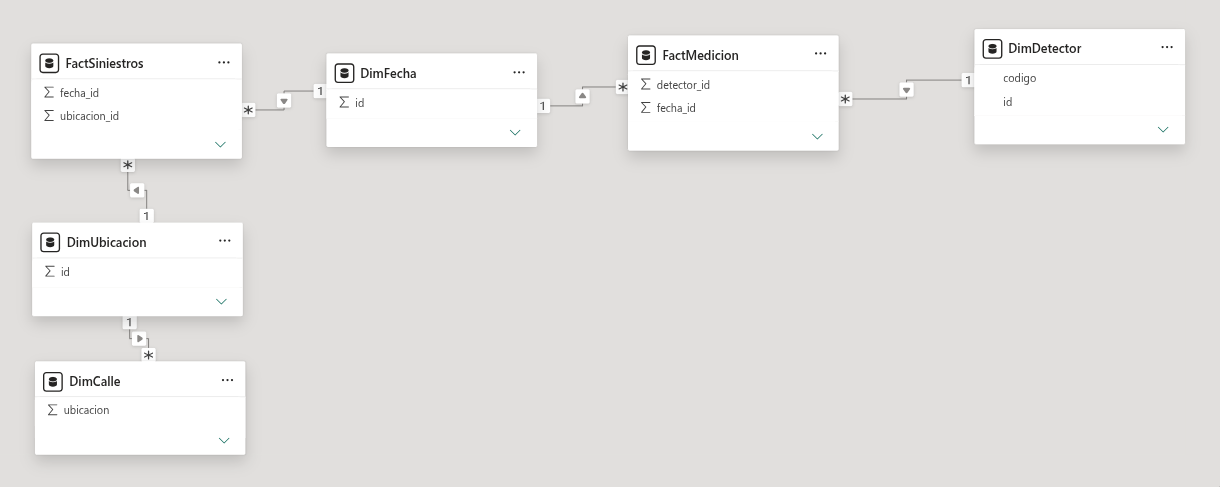
\includegraphics[scale=0.25]{graphics/diagrama-tablas.png}
    }

    \caption{Tablas finales en PowerBI}

    \label{fig:diagrama-tablas}

\end{figure}



\section{Conclusi\'on}

Este proyecto demostró que se pueden integrar datos separados de tráfico y 
siniestros usando un proceso ETL, y consolidarlos en un modelo de esquema de 
constelación. El principal valor analítico del trabajo está en la creación de 
métricas clave que superan la estadística básica, como el Índice de Eficiencia 
y el Índice de Riesgo. Estos índices permitieron evaluar el flujo de las 
avenidas y su peligro real, pero siempre de forma proporcional al volumen 
vehicular. Además, el análisis del Perfil Temporal mostró claramente los 
ciclos de movilidad a lo largo de la semana y el año.

Con estas bases, el trabajo logró ofrecer un enfoque orientado a la acción con 
la categorización de Puntos Críticos y el Score de Radar, herramientas 
diseñadas para priorizar objetivamente la necesidad de fiscalización en la 
ciudad. Aunque el procesamiento de datos mostró limitaciones en las fuentes 
oficiales (formatos inconsistentes y meses sin registros), los reportes 
interactivos finales transforman esta información en una base robusta para 
respaldar la toma de decisiones en planificación y seguridad vial.



\section{Ap\'endice}

\subsection{Entrada y Salida}
\begin{lstlisting}[language=Python, caption=Tipos de Entrada (input\_types.py)]
class VelocidadPromedio:
    cod_detector: int
    id_carril: int
    fecha: datetime.date
    hora: datetime.time
    dsc_avenida: str
    dsc_int_anterior: str
    dsc_int_siguiente: str
    latitud: float
    longitud: float
    velocidad: float

class ConteoVehicular:
    cod_detector: int
    id_carril: int 
    fecha: datetime.date
    hora: datetime.time
    dsc_avenida: str
    dsc_int_anterior: str
    dsc_int_siguiente: str
    latitud: float
    longitud: float 
    volume: int
    volumen_hora: float

class Siniestros:
    fecha: datetime.date
    edad: int | None
    rol: RolEnum
    calle: str
    zona: ZonaEnum | None
    tipo_resultado: ResultadoSiniestroEnum
    tipo_siniestro: str
    usa_cinturon: bool | None
    usa_casco: bool | None
    dia_semana: str
    sexo: str | None
    hora: int
    departamento: str
    localidad: str | None
    novedad: int
    tipo_vehiculo: VehiculoEnum | None
    fixed: str | None
    x: int
    y: int
\end{lstlisting}

\begin{lstlisting}[language=python, caption=Tipos de Salida (output\_types.py)]
class dim_fecha:
    id: int
    fecha: datetime.date
    anio: int
    mes: int
    dia: int

class dim_ubicacion:
    id: int 
    latitud: float
    longitud: float
    descripcion: str
    tipo: str

class dim_calle:
    id: int 
    ubicacion: int 
    nombre: str

class dim_detector:
    id: int 
    codigo: int 
    avenida: str
    int_anterior: str
    int_siguiente: str
    latitud: float
    longitud: float

class fact_medicion:
    fecha_id: int
    detector_id: int 
    hora: datetime.time 
    id_carril: int
    velocidad: float
    volumen: int
    volumen_hora: int

class fact_siniestros:
    fecha_id: int
    ubicacion_id: int 
    tipo_resultado: ResultadoSiniestroEnum
    tipo_siniestro: str
    usa_cinturon: bool | None
    usa_casco: bool | None
    edad: int
    sexo: str | None

\end{lstlisting}


% \bibliographystyle{plain} 
% \bibliography{Referencias}

\end{document}



